\section{Divide et Impera}
Il metodo Divide et Impera, non ha memoria, ogni volta che si calcola una soluzione, il processo richiede di ricalcolare la sottoistanza del problema che lo ha risolto, generando quindi un problema di sottoistanze ripetute. \\~\\

Il Divide et Impera, possiede 2 fasi:
\begin{itemize}
    \item \textbf{Top-down:} con cui vengono generate le istanze risolte divide il problema originale in un numero di sottoproblema (divide), risolvendo i problemi ricorsivamente (impera) e combinando le soluzioni dei sottoproblemi nella soluzione ai sottoproblemi originali (combine)
    \item \textbf{Bottom-up:} normalmente non ricorsiva ma iterativa
    \begin{itemize}
        \item caratterizza la struttura delle soluzioni ottimali
        \item definiscono ricorsivamente i valori delle soluzioni ottimali
        \item calcola il valore delle soluzioni ottimali
        \item costruisce una soluzione ottimale a partire dalle informazioni calcolate
    \end{itemize}
    Sinteticamente, si elaborano le soluzioni alle istanze presenti.
\end{itemize}
\begin{center}
    \begin{tabular}{c}
        \\ 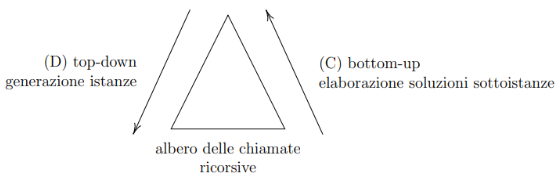
\includegraphics[width=0.8\textwidth]{image/T-D_B-U.png} \\ \\
    \end{tabular}
\end{center}
L'approccio della programmazione dinamica salta completamente l'approccio top-down, normalmente usando algoritmi iterativi per evitare di dover calcolare la soluzione. La programmazione Divide et Impera usa entrambi gli approcci e normalmente in modo ricorsivo.

\subsection{Memoizzazione}
È possibile mantenere i vantaggi del Top-down e quindi anche del Divide et Impera senza incorrere nel problema del ricalcolo delle soluzioni, usando il concetto di memoizzazione. \\~\\

Un algoritmo memoizzato è costituito da 2 subroutine/procedure:
\begin{itemize}
    \item \textbf{routine di inizializzazione:}
    \begin{itemize}
        \item risolve direttamente i casi base
        \item inizializza una struttura dati "tabella" che contiene le soluzioni ai casi base ed elementi per tutte le sottoistanze da calcolare inizializzate ad un valore di default
        \item invoca la struttura ricorsiva
    \end{itemize}
    \item \textbf{routine ricorsiva:}
    \begin{itemize}
        \item segue il codice del Divide et Impera preceduto da un test sulla tabella per verificare se la soluzione è già stata calcolata e memorizzata
        \item se si, ritorna
        \item altrimenti si calcola ricorsivamente e si memorizza nella struttura
    \end{itemize}
\end{itemize}

\subsection{Ottimizzazione}
Ora, consideriamo i problemi di ottimizzazione, per cui si cerca di trovare una cosiddetta soluzione ottima, definita come $s*$, definendo tutto come segue:
\begin{itemize}
    \item $I =$ insieme delle istanze
    \item $S =$ insieme delle soluzioni
    \item $\forall i \in I, S(i) = \{s \in S: (i,s) \in \Pi\} =$ insieme delle soluzioni ammissibili
    \item $c: S \rightarrow \mathbb{R} =$ funzione di costo
    \item $i \in I, s* \in S(i): c(s*) = \min / \max \{c(s): s \in S(i)\}$
\end{itemize}

Paradigma generale sullo sviluppo di un algoritmo di programmazione dinamica. Caratteristiche dei problemi:
\begin{itemize}
    \item struttura ricorsiva: la soluzione ottima si ottiene come funzione di soluzioni ottime di sottoistanze ("proprietà di sottostruttura ottima", quindi il fatto che ogni soluzione contenga già soluzioni precedenti)
    \item esistenza di sottoistanze ripetute ("overlapping subproblems"), teoricamente risolvibili in maniera ottima (altrimenti, conviene applicare Divide et Impera)
    \item spazio dei sottoproblemi piccolo: poche sottoistanze che possono contribuire a crearela soluzione al livello superiore
\end{itemize}

Ricetta:
\begin{itemize}
    \item caratterizza la struttura di una soluzione ottima $s*$ in funzione di soluzioni ottime $s_1*, \ldots, s_k*$ di sottoistanze di taglia inferiore
    \item determinare una relazione di ricorrenza del tipo $c(s*) = f(c(s_1*), \ldots, c(s_k*))$
    \item calcola $C(S*)$ utilizzando la ricorrenza ma impostando il calcolo in maniera bottom-up (iterativo) oppure memoizzando il codice Divide et Impera basato sulla definizione di $C(S*)$
    \item (opzionale) mantieni informazioni strutturali aggiuntive che permettono di ricostruire $S*$
\end{itemize}

\newpage
\subsection{Problemi su stringhe}
\begin{mdframed}
    \textbf{Def} Dato un alfabeto finito $\sum$, una stringa
    \begin{equation*}
        X = \langle x_1, x_2, \ldots, x_m \rangle, x_i \in \sum \quad \forall\; 1 \leq i \leq m
    \end{equation*}
    è una concetazione finita di simboli in $\sum$
    \begin{itemize}
        \item $m = |X| =$ lunghezza di $X$
        \item $\sum* =$ insieme di tutte le stringhe di lunghezza finita costruibili su $\sum$
        \item $\varepsilon$ = stringa vuota
    \end{itemize}
    Data una stringa $X$, il prefisso di $X$ è
    \begin{equation*}
        X_i = \langle x_1, x_2, \ldots, x_i \rangle 1 \leq i \leq m
    \end{equation*}
    Data una stringa $X$, il suffisso di $X$ è
    \begin{equation*}
        X^i = \langle x_i, x_{i+1}, \ldots, x_m \rangle 1 \leq i \leq m
    \end{equation*}
    Per convenzione: $X_0 = X^{m+1} = \varepsilon$
\end{mdframed}

\begin{mdframed}
    \textbf{Def} Data una stringa $X$, la sottostringa di $X$ è
    \begin{equation*}
        X_{i \ldots j} = \langle x_i, x_{i+1}, \ldots, x_j \rangle \quad 1 \leq i \leq j \leq m
    \end{equation*}
    Per convenzione: $X_i \ldots j = \varepsilon \quad (i > j)$
\end{mdframed}

\begin{mdframed}
    \textbf{Def} Data una stringa
    \begin{equation*}
        X = \langle x_1, x_2, \ldots, x_m \rangle \in \sum*
    \end{equation*}
    \begin{equation*}
        Z = \langle z_1, z_2, \ldots, z_k \rangle \in \sum*
    \end{equation*}
    si dice che $Z$ è sottosequenza di $X$ se $\exists$ una successione crescente di indici
    \begin{equation*}
        1 \leq i_1 \leq i_2 \leq \ldots \leq i_k \leq m: z_j = x_{ij} \quad \forall\; 1 \leq j \leq k
    \end{equation*}
\end{mdframed}

\newpage
